\documentclass[hyperref]{beamer}
\usepackage{beamerthemesplit}
\usepackage{graphicx}
\usepackage{mathptmx}           % replacement for obsolete \usepackage{times}
\usepackage[scaled=1.0]{helvet} % replacement for obsolete \usepackage{times}
\usepackage{courier}            % replacement for obsolete \usepackage{times}
\usepackage[normalem]{ulem}


\usepackage{tikz}
\usepackage{../tikz-dependency,pifont}
\usetikzlibrary{shapes.arrows,chains,positioning,automata,trees,calc}
\usetikzlibrary{patterns}
\usetikzlibrary{decorations.pathmorphing,decorations.markings}
\usepackage{times,latexsym,amsfonts,amssymb,amsmath,graphicx,url,bbm,rotating,siunitx}
\usepackage{multirow,hhline,arydshln,array,color,stmaryrd,pifont,transparent}
\usepackage[absolute,overlay]{textpos}
\definecolor{darkred}{rgb}{0.5, 0.0, 0.0}
\definecolor{darkgreen}{rgb}{0.0, 0.4, 0.0}
\definecolor{darkblue}{rgb}{0.0, 0.0, 0.5}

% set up Beamer style with Stanford colors and logo
% logo is available at http://nlp.stanford.edu/local/nlp-logos/nlp-logo.pdf
\useinnertheme{rounded}
\useoutertheme{infolines}
\usecolortheme{beaver}
\setbeamercolor{block title}{fg=white,bg=darkred!75!black}
\setbeamercolor{block body}{parent=normal text,bg=black!5!bg}
\setbeamercolor{item projected}{bg=darkred}
\setbeamertemplate{enumerate items}[default]
\logo{
\includegraphics[height=1cm]{../img/nlp-logo.pdf}}

% title page information
\title[Gabor's Thesis Proposal]{Natural Language Inference for Question Answering}
\subtitle{}
\author{Gabor Angeli}
\date{April 14, 2015}
\institute[Stanford]{Stanford University}

\input ../macros.tex
\input ../figures_naturalli.tex
\input ../figures_kbp.tex

\begin{document}
\begin{frame}[noframenumbering]
  \titlepage
\end{frame}

\input abstract.tex
\input kbp.tex
\input openie.tex
\input natlog.tex
\input naturalli.tex
\input future.tex


%%%%%%%%%%%%%%%%%%% 
% THANKS
%%%%%%%%%%%%%%%%%%%
\begin{frame}[noframenumbering]{}
\begin{center}
  \hh{\huge{Thanks!}} \\
  \vspace{1cm}
  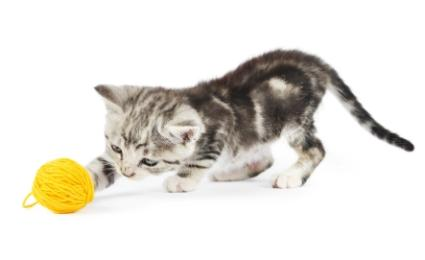
\includegraphics[width=3cm]{../img/yarn-cat.jpg} \\
%  \vspace{1cm}
%  \url{http://plato42.stanford.edu/naturalli}
\end{center}
\end{frame}



\begin{frame}[allowframebreaks]
  \frametitle{References}
  \bibliographystyle{apalike}
  \bibliography{../ref}
\end{frame}

\end{document}
